\documentclass[11pt]{article}
\usepackage[margin=1in]{geometry}
\usepackage{graphicx}
\newcommand{\SampleSize}{32}
\newcommand{\ModelRsquared}{0.827}
\newcommand{\WeightEstimate}{-3.878}

\title{A Reproducible R Workflow: A Teaching Example}
\author{Course example}
\date{}
\begin{document}
\maketitle
\section{Data and methods}
The built-in R dataset \texttt{mtcars} contains \SampleSize{} cars.
We fit ordinary least squares regression of fuel economy (mpg) on
weight (1000 lbs) and horsepower. This is an observational teaching example.
\section{Results}
The model has $R^2=\ModelRsquared$.
The adjusted association for weight is \WeightEstimate{} mpg per 1000 lbs.
This association is not a causal effect.
\begin{table}[htbp]
\centering
\caption{Model coefficients with conventional linear-model uncertainty.}
\begin{tabular}{lrrrr}
\hline
Term & Estimate & SE & 95\% CI & $p$ \\
\hline
Intercept & 37.227 & 1.599 & [33.957, 40.497] & $<0.001$ \\
Weight (1000 lbs) & -3.878 & 0.633 & [-5.172, -2.584] & $<0.001$ \\
Horsepower & -0.032 & 0.009 & [-0.050, -0.013] & 0.001 \\
\hline
\end{tabular}

\end{table}
\begin{figure}[htbp]
\centering
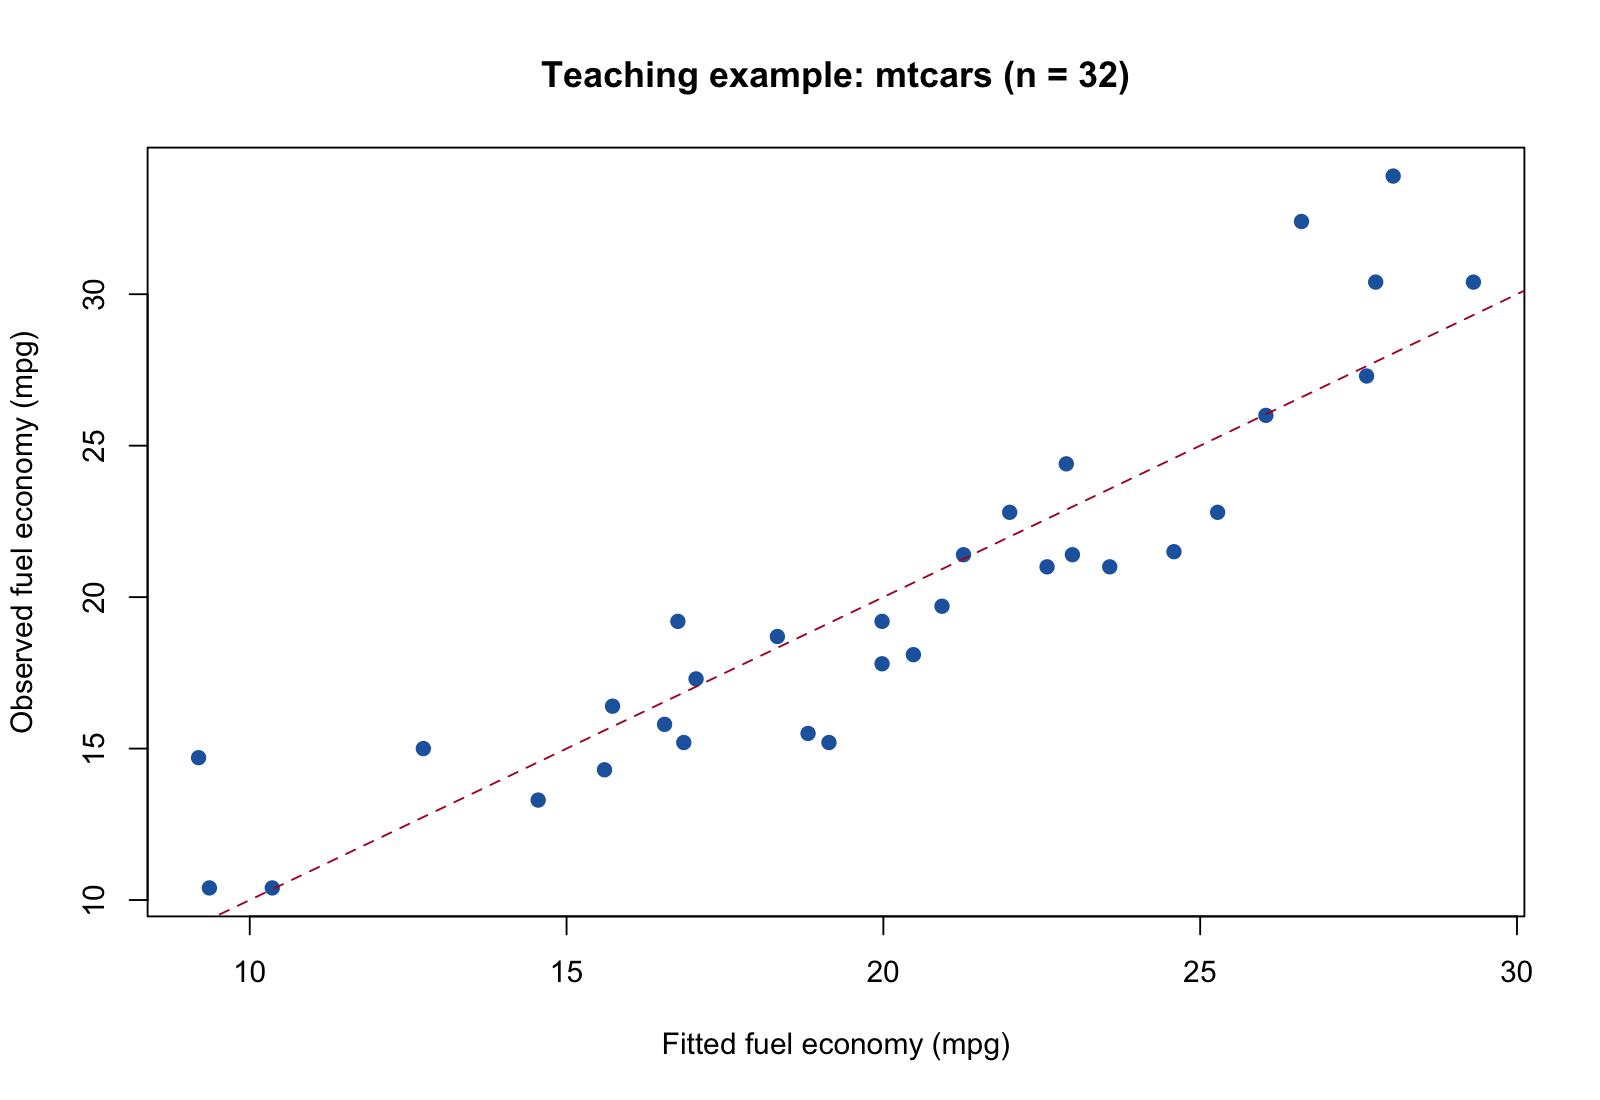
\includegraphics[width=0.8\linewidth]{../outputs/figures/observed-fitted.pdf}
\caption{Observed and fitted fuel economy; the dashed line denotes equality.}
\end{figure}
\section{Limitations and reproducibility}
The small sample and model assumptions limit inference. Residual and influence
diagnostics are needed before substantive interpretation. Run \texttt{Rscript run.R}
from the project root to regenerate all reported numbers and graphics.
\end{document}
